% 编译方式：在报告目录运行 xelatex main.tex（目录更新需编译两次）
\documentclass[UTF8,a4paper,12pt]{ctexart}
\usepackage[margin=2.5cm]{geometry}
\usepackage{amsmath,amssymb}
\usepackage{graphicx}
\usepackage{booktabs}
\usepackage{array}
\usepackage{float}
\usepackage{hyperref}
\hypersetup{hidelinks}
\setlength{\parindent}{2em}
\setlength{\parskip}{0.3em}
\linespread{1.3}
% 将图片放在报告目录下的 figures 文件夹，取消对应代码的注释即可插入。
\graphicspath{{figures/}}
\newcommand{\todo}[1]{\textit{［待填写：#1］}}

\begin{document}
\begin{center}
  {\LARGE\bfseries 光盘光谱仪\par}

  \vspace{1em}
  参赛人姓名：\todo{姓名}\\
  学号：\todo{学号}\\
  所在学院／专业：\todo{学院及专业}
\end{center}
% 多位成员可逐行填写姓名、学号和学院／专业。
\setcounter{tocdepth}{1}
\tableofcontents
\newpage

\section{题目介绍}
Data tracks on optical media (e.g. CDs / Blu-ray discs) behave as high-quality reflection-diffraction gratings. When illuminated, these discs can disperse light into its spectral components. Construct a spectrometer using a digital optical disc. Optimise the design to maximise the resolving power and minimise optical aberrations.

光学存储介质（如 CD 或蓝光光盘）上的数据轨道可以作为反射式衍射光栅。当受到光照时，光盘能将光色散成其光谱成分。本课题要求利用数字光盘构建光谱仪，并优化其设计，以提高分辨本领、减小光学像差。

\todo{简述本队的研究问题、研究对象及工作范围。}
那么我们需要就是先确定光谱仪结构, 再去探究各种因素对分辨率的影响, 综合考虑各个因素后, 得到兼顾性价比与分辨率的设计结构


\section{课题研究背景}
\subsection{研究背景与意义}
光谱是物质与电磁辐射相互作用后形成的特征信息。不同物质在不同波长处具有不同的吸收、发射或反射特征，因此对光谱进行测量和分析，可以用于识别物质成分、研究材料性质、监测化学反应过程，以及排查大气和水体中的污染物等\cite{yuan2023,wang2025,yang2021}。光谱仪将不同波长的光分开并记录其强度分布，是获取这类信息的重要工具。

传统光谱仪通常使用棱镜或衍射光栅等色散元件。衍射光栅通过周期性结构使不同波长的光沿不同方向传播，具有色散能力强、结构原理清楚等特点；但是传统光谱仪往往价格昂贵，限制了日常可及性,因此有必要开发经济实惠的替代方案。

数字光盘的数据轨道具有规则的周期结构，可作为反射式衍射光栅使用,有助于推动光谱仪的普及化和低成本化。
\subsection{前人研究进展}
光谱仪能够测量光强随波长的分布，在物理、化学、生物和环境科学等领域有广泛应用。为满足教学和低成本研究的需要，研究者探索了使用常见光学元件、图像传感器和开源软硬件搭建光谱仪的方案。这些方案在降低成本的同时，也需要处理波长标定、光学装调、探测范围和分辨能力等问题。

da Silva 等设计了一种低成本光谱仪，采用图像传感器、光栅和嵌入式计算平台采集并处理光谱信息\cite{dasilva2018}。Hong 和 Sengupta 则研究了面向可见光和近红外波段的 CMOS 集成光谱仪\cite{hong2017}。这些工作体现了利用电子图像传感器与计算处理实现光谱测量的不同思路。Nikita 等在其引言中指出，低成本装置仍需关注波长范围、灵敏度与标定等因素\cite{nikita2025spectrometer}。

在采用日常材料的方案中，Likith 等研究了面向传感应用的低成本光谱仪\cite{likith2021}。Nikita 等介绍，该类简易装置可以使用纸板、DVD 和网络摄像头等材料，但装置的机械稳定性、光路对准以及图像处理方式都可能影响测量结果；摄像头自身的光谱响应和滤光结构也会限制可测波段\cite{nikita2025spectrometer}。因此，使用低成本器材时，除观察到色散现象外，还需要验证波长标定和测量结果的可靠性。

在便携式光谱仪方面，Nikita 等还综述了以智能手机作为图像采集平台、配合光栅薄膜或微机电系统光栅的方案。引言同时介绍了采用光纤、CCD 探测器、全息光栅以及树莓派与线阵 CCD 的设计，并讨论了它们在便携性、成本、装调复杂度和性能方面的不同取舍\cite{nikita2025spectrometer}。这些案例表明，色散元件、探测器和机械结构需要共同设计，才能获得满足目标的光谱质量。

基于上述思路，Nikita 等提出了一种由 DVD 光栅、网络摄像头和 Python 程序构成的低成本光谱仪，并使用遮光箱减少环境杂散光。该工作利用商用光纤光谱仪辅助标定，并对多种 LED 光源和激光器的光谱进行测量和比较\cite{nikita2025spectrometer}。这一方案为利用光盘构建光谱仪提供了参考，也提示我们需要关注遮光、标定和图像采集等环节。

已有工作展示了低成本光谱测量的可行性，但峰值波长与参考仪器接近，不能直接说明装置分辨相邻谱线的能力。本课题将围绕光盘光栅及实际光路，进一步研究光盘类型、照明区域、狭缝与成像条件等因素对谱线宽度和像差的影响，以探索兼顾分辨能力与器材成本的设计。
\subsubsection{高分辨率光谱仪：F--P 干涉仪与光栅联用}
当需要区分波长非常接近的谱线时，可以将具有高光谱选择性的干涉器件与色散元件联用。以法布里--珀罗（Fabry--Pérot，简称 F--P）干涉仪为例，光在两反射面之间多次反射，多个出射光束相干叠加，使透射光谱出现一系列较窄的周期性透射峰。改变两反射面之间的间距，可以移动透射峰的位置，逐步扫描待测光谱。

F--P 干涉仪的相邻透射峰之间具有有限的自由光谱范围。宽波段光同时入射时，不同干涉级次可能产生多个透射峰，仅靠单次透射信号难以确定各峰对应的波长。将 F--P 干涉仪与光栅光谱仪级联后，光栅可以在空间上区分不同波长区域的透射信号；通过扫描腔长并记录各位置的光强，再进行光谱重构，可以兼顾较宽的测量范围与较高的光谱分辨能力。该方法要求合理匹配 F--P 干涉仪的自由光谱范围和光栅光谱仪的分辨能力，并考虑扫描时间与标定等因素\cite{zhong2020micro}。

钟卉提出了可调谐微型 F--P 干涉仪与微型曲面光栅光谱仪级联的设计，并以拉曼光谱仪为例进行光学设计和光谱重构仿真。论文给出的拉曼位移范围为 $150$--$3200\,\mathrm{cm}^{-1}$，重构光谱的分辨率约为 $6.4\,\mathrm{cm}^{-1}$；这些数值来自设计与仿真，不是本课题装置的实测结果\cite{zhong2020micro}。这一方案展示了干涉滤波和光栅色散的互补作用，也为理解高分辨率与宽光谱范围之间的设计取舍提供了参考。
\section{预实验现象}
\subsection{预实验方法与现象}
\todo{记录预实验所用光源、光盘和观察方法，描述实际观察到的现象。}
\subsection{预实验图片}
\todo{插入本人拍摄的预实验图片，说明拍摄条件和图中现象。}
% \begin{figure}[H]
%   \centering
%   \includegraphics[width=0.75\textwidth]{preliminary.jpg}
%   \caption{预实验现象（请补充具体说明）}
%   \label{fig:preliminary}
% \end{figure}

\section{理论分析}
\subsection{光栅衍射的物理机理}
数字光盘上的数据轨道近似周期排列，光照射到盘面后，相邻轨道反射的光在空间中相干叠加。由于不同方向上相邻轨道产生的光程差不同，某些方向的光相长干涉，形成各级衍射光。不同波长对应的相长干涉方向不同，因此复色光经过光盘后会产生色散。

在照明区域足够小、轨道间距近似不变时，可以将局部盘面视为平面反射光栅。设光栅周期为 $d$，入射光和衍射光均位于垂直于局部轨道的平面内。以光栅表面法线为基准，将从光栅指向光源和从光栅指向观察方向的角度分别记为 $\alpha$ 和 $\beta$；两角以法线同一侧为正、另一侧为负。相邻轨道的光程差为 $d(\sin\alpha+\sin\beta)$，相长干涉条件给出反射光栅方程
\begin{equation}
  d(\sin\alpha+\sin\beta)=m\lambda,
  \label{eq:grating}
\end{equation}
其中 $\lambda$ 为光在周围介质中的波长，$m=0,\pm1,\pm2,\ldots$ 为衍射级次。对确定的入射角和波长，只有满足 $|m\lambda/d-\sin\alpha|\leq 1$ 的级次才存在对应的传播方向。零级光满足 $\beta=-\alpha$，对应镜面反射方向；非零级次中，不同波长的衍射角不同。

固定入射角和衍射级次，对式\eqref{eq:grating}求导，可得角线色散率
\begin{equation}
  \frac{\mathrm{d}\beta}{\mathrm{d}\lambda}=\frac{m}{d\cos\beta}.
  \label{eq:angular-dispersion}
\end{equation}
其绝对值表示单位波长变化引起的衍射角变化。若成像透镜在近轴条件下将小角度差转化为焦平面上的位置差，则线色散率可近似写为 $|\mathrm{d}x/\mathrm{d}\lambda|\approx f|\mathrm{d}\beta/\mathrm{d}\lambda|$，其中 $f$ 为成像透镜焦距。光栅轨道间距、工作级次、入射角和成像条件共同决定探测器上的光谱展开情况。

\subsection{光谱分辨率与分辨本领}
光谱分辨率 $\Delta\lambda$ 通常表示在给定判据和测量条件下能够区分的最小波长间隔；分辨本领定义为
\begin{equation}
  R=\frac{\lambda}{\Delta\lambda}.
\end{equation}
对于均匀照明、周期规则的理想光栅，在瑞利判据下有
\begin{equation}
  R=|m|N,
\end{equation}
其中 $N$ 为受到有效照明的光栅周期数。实际光谱仪的分辨能力还受到狭缝宽度、光束准直、像差、探测器采样和光盘轨道曲率等因素影响，需要通过谱线测量评价。
\subsection{自由光谱范围与衍射级次重叠}
光栅将不同波长的光按衍射角分开，但同一波长可以出现在多个衍射级次中。如图\ref{fig:grating-fsr}所示，每一个级次都形成一组光谱；当入射光的波长范围较宽时，相邻级次的光谱可能在同一方向重叠。此时，探测器在该方向接收到的光可能来自不同波长和不同级次，仅根据衍射角无法唯一确定波长。

\begin{figure}[H]
  \centering
  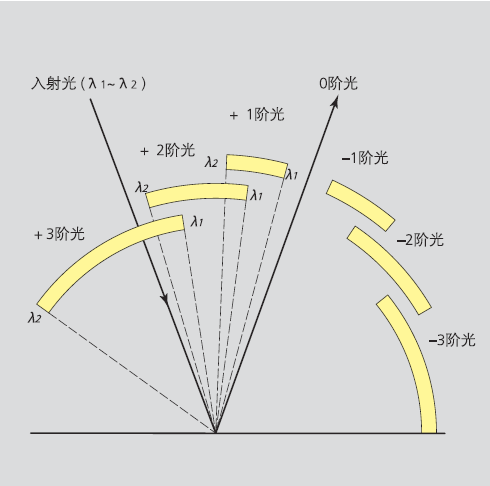
\includegraphics[width=0.65\textwidth]{fig/fsr.png}
  \caption{不同衍射级次的光谱分布示意图}
  \label{fig:grating-fsr}
\end{figure}

在固定入射角和观察方向下，光栅衍射条件要求 $m\lambda$ 为定值。因此，级次 $m$ 中波长为 $\lambda$ 的光与级次 $m+1$ 中波长为 $\lambda'$ 的光重合时，有
\begin{equation}
  m\lambda=(m+1)\lambda'.
\end{equation}
这里 $m$ 为正整数，$\lambda>\lambda'$。对应的波长间隔称为该波长附近的自由光谱范围：
\begin{equation}
  \Delta\lambda_{\mathrm{FSR}}=\lambda-\lambda'
  =\frac{\lambda}{m+1}
\end{equation}
自由光谱范围描述的是避免相邻级次重叠所对应的波长间隔，它与分辨相近谱线的能力是两个不同的指标。实际仪器可通过限制入射波段或使用滤光片等方式抑制级次重叠。


\subsection{理论建模}
\todo{写出所采用的模型、主要假设、公式及各物理量的含义；讨论分辨本领与像差的影响因素。}
\subsection{计算与模拟结果}
\todo{说明计算或模拟方法、参数及结果，加入必要的图表，并注明其适用范围。}

\section{实验装置}
\subsection{装置组成与光路}
\todo{介绍光源、狭缝、准直和成像元件、光盘、探测器等实际使用的部件及其连接方式。}
\subsection{装置图片}
\todo{插入实际搭建装置的照片，并标注主要部件；可另附光路示意图。}
% \begin{figure}[H]
%   \centering
%   \includegraphics[width=0.75\textwidth]{apparatus.jpg}
%   \caption{实验装置实物图（请补充部件说明）}
%   \label{fig:apparatus}
% \end{figure}

\section{实验分析}
\subsection{实验步骤与测量方法}
\todo{按实际操作顺序说明装调、标定、测量及数据处理方法，列出控制变量。}
\subsection{实验测量数据}
\todo{填写原始数据或汇总数据、单位、测量条件及必要的不确定度。}
% 根据实际测量量修改表头和行数。
\begin{table}[H]
  \centering
  \caption{实验测量数据（待补充）}
  \begin{tabular}{ccc}
    \toprule
    测量条件 & 测量量及单位 & 备注 \\
    \midrule
    待填写 & 待填写 & 待填写 \\
    \bottomrule
  \end{tabular}
\end{table}
\subsection{实验结果分析}
\todo{展示处理后的结果，分析分辨本领、像差和不同条件的影响，并讨论误差及不确定度。}

\section{研究结论}
\subsection{理论分析结论}
\todo{概括理论分析或模拟所得的主要结论及其适用条件。}
\subsection{实验结论}
\todo{根据实际测量结果概括主要发现，给出有数据支持的结论。}
\subsection{理论与实验对比}
\todo{比较理论预测与实验结果，分析差异及可能原因。}

\section{团队分工}
\todo{逐一填写每位成员承担的具体工作。}
\begin{table}[H]
  \centering
  \begin{tabular}{p{0.2\textwidth}p{0.65\textwidth}}
    \toprule
    成员 & 具体分工 \\
    \midrule
    待填写 & 待填写 \\
    \bottomrule
  \end{tabular}
\end{table}

\begin{thebibliography}{99}
\bibitem{yuan2023} Yuan S F, Ma C, Fetaya E, Mueller T, Naveh D, Zhang F, Xia F N. \textit{Science}, 2023, 379(6637).
\bibitem{wang2025} Wang F K, Fang S, Zhang Y, Wang Q J. \textit{Nature Communications}, 2025, 16: 6791.
\bibitem{yang2021} Yang Z Y, Albrow-Owen T, Cai W W, Hasan T. \textit{Science}, 2021, 371(6528).
\bibitem{singh1999gratings} Singh S. Diffraction gratings: aberrations and applications[J]. \textit{Optics and Laser Technology}, 1999, 31(3): 195--218.
\bibitem{nikita2025spectrometer} Nikita Z J, Alam M T, Mahmud Y, et al. Developing a Cost-Effective Spectrometer: A Practical Approach[EB/OL]. arXiv:2510.06703v4, 2025. \url{https://arxiv.org/abs/2510.06703v4}.
\bibitem{dasilva2018} da Silva M, Panda S, Tiwari D, Nair S, Jadhav A. Design and implementation of low cost optical spectrometer[C]. ICICCT, 2018: 1904--1908. \url{https://doi.org/10.1109/ICICCT.2018.8473130}.
\bibitem{hong2017} Hong L, Sengupta K. Fully integrated optical spectrometer in visible and near-IR in CMOS[J]. \textit{IEEE Transactions on Biomedical Circuits and Systems}, 2017, 11(6): 1176--1191. \url{https://doi.org/10.1109/TBCAS.2017.2774603}.
\bibitem{likith2021} Likith G, Jayram N D, Yaswanth B, et al. Designing of low-cost spectrometer for sensor application[J]. \textit{Journal of Optics}, 2021, 50: 489--494. \url{https://doi.org/10.1007/s12596-021-00707-w}.
\bibitem{zhong2020micro} 钟卉. 高分辨率宽光谱范围微型光谱仪的设计与分析[J]. \textit{激光与光电子学进展}, 2020, 57(15): 153004. \url{https://doi.org/10.3788/LOP57.153004}.
\end{thebibliography}
\end{document}












